%!TEX root = thesis.tex


\chapter{SWEET-Cat}
\label{sec:SWEET-Cat}

\section{Parameters for 50 planet hosts}



The method of determining atmospheric parameters from the curve of growth analysis has been applied
several times in the optical \citep[see e.g.][]{Mortier2013b,Tsantaki2013,Sousa2011,Santos2013}.
When studying stars with planets and any correlations between stellar and planetary parameters it is
important to have a homogeneous characterisation of the stars. An effort to create such a sample was
initiated by \citet{Santos2013} with the SWEET-Cat
database\footnote{\url{https://www.astro.up.pt/resources/sweet-cat/}}. The motivation to homogenise
the stellar hosts is mainly to compare the hosts and make statistical studies on one consistent
scale. When doing these statistical studies, the results might otherwise suffer from offsets between
different methods.

The skills acquired during the NIR studies as mentioned above were directly translated into deriving
parameters for a sample of 50 known planet host stars that were not previously analysed by our group
\citep{Andreasen2017a}. The spectra of these stars were required at UVES, FIES, HARPS, and ESPaDOnS
with the mean S/N higher than 200\unfinished{Write more about the data acquisition here}.

A Hertzsprung-Russell diagram of the sample can be seen in \fref{fig:sweetcat}. The sample covers a
large range of $T_\mathrm{eff}$, FGK, while there are both dwarf, sub-giant, and some giant stars.
The colours indicate the $\log g$. In order to determine the luminosity of each star the simple
relation
\begin{align*}
  L = 4\pi R^2 \sigma T^4_\mathrm{eff}
\end{align*}
is used, where $L$ is the luminosity, $R$ is the stellar radius, and $\sigma$ is the
Stefan-Boltzmann constant. In solar units this relation is simply:
\begin{align*}
  \frac{L}{L_\odot} = \left(\frac{R}{R_\odot}\right)^2 \left(\frac{T_\mathrm{eff}}{T_{\mathrm{eff},\odot}}\right)^4
\end{align*}
In order to determine the the stellar radius, the empirical relation from \citet{Torres2010} was
used.

\begin{figure}[htpb!]
    \centering
    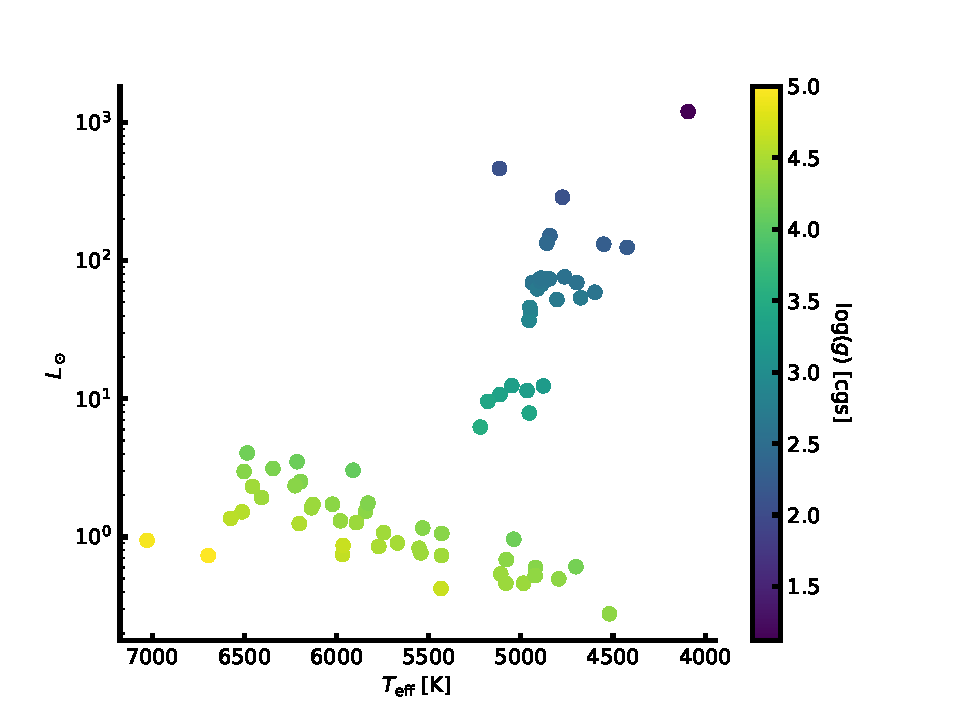
\includegraphics[width=1.0\linewidth]{figures/HR.pdf}
    \caption{A Hertzsprung-Russell diagram of the sample of 50 planet host stars added to SWEET-Cat.
             The parameters were derived using optical high resolution and high S/N spectra in
             tandem with \FASMA and an optical line list. The colour scale shows the derived
             $\log g$ for each star.}
    \label{fig:sweetcat}
\end{figure}

The parameters were derived using \FASMA with the optical line list compiled by \citet{Sousa2008a}
and \citet{Tsantaki2013} for stars where $T_\mathrm{eff}$ was below \SI{5200}{K}. All the new
derived parameters were added to SWEET-Cat, available for the community.

With these updated parameters the completeness of SWEET-Cat for stars brighter than V magnitude 10
is 85\% (77\% for stars brighter than 12). For fainter stars it is time expensive to acquire spectra
of the quality needed for this method. Moreover, many of the fainter planet host stars have been
observed with the \emph{Kepler} space mission, where most stars are faint.

SWEET-Cat was recently combined with planetary masses to see two distinctive populations for giant
planets by \citet{Santos2017}. This can be seen in the mass histogram in \fref{fig:giantpopulations}
for the full sample of giant planets, with masses higher than 1 Jupiter mass and lower than 20
Jupiter masses, and for a sample constrained by: $\SI{4000}{K}\leq T_\mathrm{eff} \leq\SI{6500}{K}$
in order to have reliably atmospheric parameters from spectroscopic data, orbital periods above
\SI{10}{days} to avoid hot jupiters whose formation and migration process is debated \citep[see
e.g.]{Ngo2016}, orbital periods below 5 years to allow for the sample to be reasonable complete.
Last only stars brighter than 13 magnitude were included to ensure that the planetary masses can
have been derived with reasonable confidence using the radial velocities.

\begin{figure}[htpb!]
    \centering
    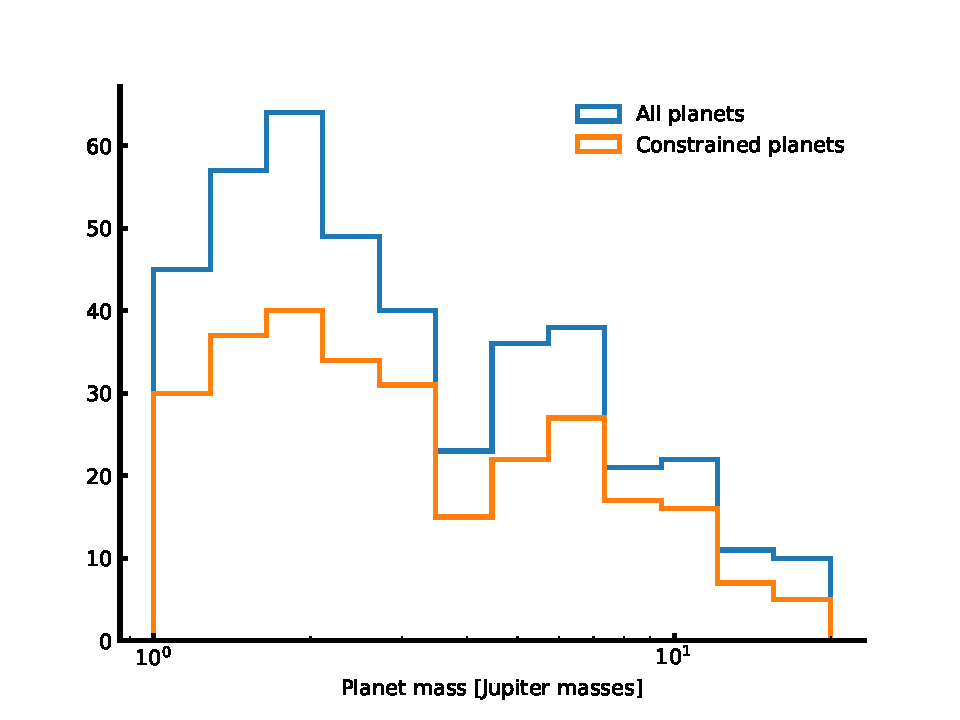
\includegraphics[width=1.0\linewidth]{figures/giantPopulation.pdf}
    \caption{Giant planet masses for the full sample and constrained sample (see text for details).
             This study was performed by \citet{Santos2017} to distinct two giant planet populations.}
    \label{fig:giantpopulations}
\end{figure}

By separating the distribution into two at $4M_{Jup}$, it can be shown \citep[see][for
details]{Santos2017} that the stars hosting the more massive giant planets are in average more
metal-poor compared to the stars hosting the lower mass giant planets. This suggest two different
stellar populations forming giant planets.
